\ifdefined\ispartofbook
\else
  % Preamble for "A Journey into Deep Learning"

% --- DOCUMENT CLASS & GEOMETRY ---
\documentclass[11pt, a4paper]{report} % Changed from 'article' to 'report' to enable \chapter command
\usepackage[margin=1in]{geometry} % Set page margins

% --- FONT & ENCODING ---
\usepackage[T1]{fontenc}
\usepackage[utf8]{inputenc}

% --- MATHEMATICS & SYMBOLS ---
\usepackage{amsmath, amssymb, amsthm} % For advanced math typesetting and theorems
\usepackage{amsfonts}                 % For math fonts
\usepackage{bm}                       % For bold math symbols

% --- GRAPHICS & TABLES ---
\usepackage{graphicx}                 % To include graphics
\usepackage{booktabs}                 % For professional-quality tables
\usepackage{caption}                  % For customizing captions

% --- LISTS & LAYOUT ---
\usepackage{enumitem}                 % For list customization
\usepackage{cases}                    % For cases environment

% --- TIKZ GRAPHICS PACKAGES (NEWLY ADDED) ---
\usepackage{tikz}
\usetikzlibrary{
    positioning,
    arrows.meta,
    fit,
    decorations.pathreplacing,
    calligraphy,
    shapes.geometric,
    shadows,
    chains,
    backgrounds % For layering
}

% --- HYPERLINKS & URLS ---
\usepackage[hyphens]{url}             % For URL formatting
\usepackage{hyperref}                 % For hyperlinks and cross-references
\hypersetup{
    colorlinks=true,
    linkcolor=blue,
    filecolor=magenta,
    urlcolor=cyan,
    citecolor=red,
}

% --- CUSTOM COMMANDS ---
\newcommand{\vect}[1]{\mathbf{#1}}
\newcommand{\matr}[1]{\mathbf{#1}}
\newcommand{\normdist}{\mathcal{N}}
\newcommand{\reals}{\mathbb{R}}
\newcommand{\E}{\mathbb{E}}

  \begin{document}
\fi

\chapter{Holistic Learning: Training Networks on Statistical Manifolds}
\label{chap:holistic_learning}

% Note: The command for the AMP Layer diagram is now included directly in chapter_7_2.tex

This chapter proposes a conceptual and theoretical shift from the standard paradigm of stochastic, mini-batch-based training. We will explore the author's intention to evolve a neural network by operating directly on the statistical properties of the entire dataset, modeled as a single, high-dimensional Gaussian distribution. This approach reframes learning not as an iterative process of correcting errors from small samples, but as a holistic optimization of the network's transformation of one statistical manifold (the input distribution) to another (the target distribution). This chapter will lay the groundwork for understanding Analytical Moment Propagation and its implications for a more deterministic and principled view of deep learning.

% --- Include Subchapters ---
\ifdefined\ispartofbook
\else
  % Preamble for "A Journey into Deep Learning"

% --- DOCUMENT CLASS & GEOMETRY ---
\documentclass[11pt, a4paper]{report} % Changed from 'article' to 'report' to enable \chapter command
\usepackage[margin=1in]{geometry} % Set page margins

% --- FONT & ENCODING ---
\usepackage[T1]{fontenc}
\usepackage[utf8]{inputenc}

% --- MATHEMATICS & SYMBOLS ---
\usepackage{amsmath, amssymb, amsthm} % For advanced math typesetting and theorems
\usepackage{amsfonts}                 % For math fonts
\usepackage{bm}                       % For bold math symbols

% --- GRAPHICS & TABLES ---
\usepackage{graphicx}                 % To include graphics
\usepackage{booktabs}                 % For professional-quality tables
\usepackage{caption}                  % For customizing captions

% --- LISTS & LAYOUT ---
\usepackage{enumitem}                 % For list customization
\usepackage{cases}                    % For cases environment

% --- TIKZ GRAPHICS PACKAGES (NEWLY ADDED) ---
\usepackage{tikz}
\usetikzlibrary{
    positioning,
    arrows.meta,
    fit,
    decorations.pathreplacing,
    calligraphy,
    shapes.geometric,
    shadows,
    chains,
    backgrounds % For layering
}

% --- HYPERLINKS & URLS ---
\usepackage[hyphens]{url}             % For URL formatting
\usepackage{hyperref}                 % For hyperlinks and cross-references
\hypersetup{
    colorlinks=true,
    linkcolor=blue,
    filecolor=magenta,
    urlcolor=cyan,
    citecolor=red,
}

% --- CUSTOM COMMANDS ---
\newcommand{\vect}[1]{\mathbf{#1}}
\newcommand{\matr}[1]{\mathbf{#1}}
\newcommand{\normdist}{\mathcal{N}}
\newcommand{\reals}{\mathbb{R}}
\newcommand{\E}{\mathbb{E}}

  \begin{document}
  \input{Image_CombinedDiagram.tex} % For standalone compilation
  % This file defines the command for the combined forward/backward pass diagram.
% It can be compiled standalone or included in a larger document.

\ifdefined\ispartofbook
\else
  % --- Standalone Compilation Preamble ---
  \documentclass[tikz, border=10pt]{standalone}
  \usepackage{amsmath, amssymb} % For math symbols
  \usepackage{tikz}
  \usetikzlibrary{
    positioning,
    arrows.meta,
    fit,
    decorations.pathreplacing,
    calligraphy,
    shapes.geometric,
    shadows,
    chains,
    backgrounds
  }
  \begin{document}
\fi

% --- THE DIAGRAM COMMAND ---
\newcommand{\combineddiagram}{%
    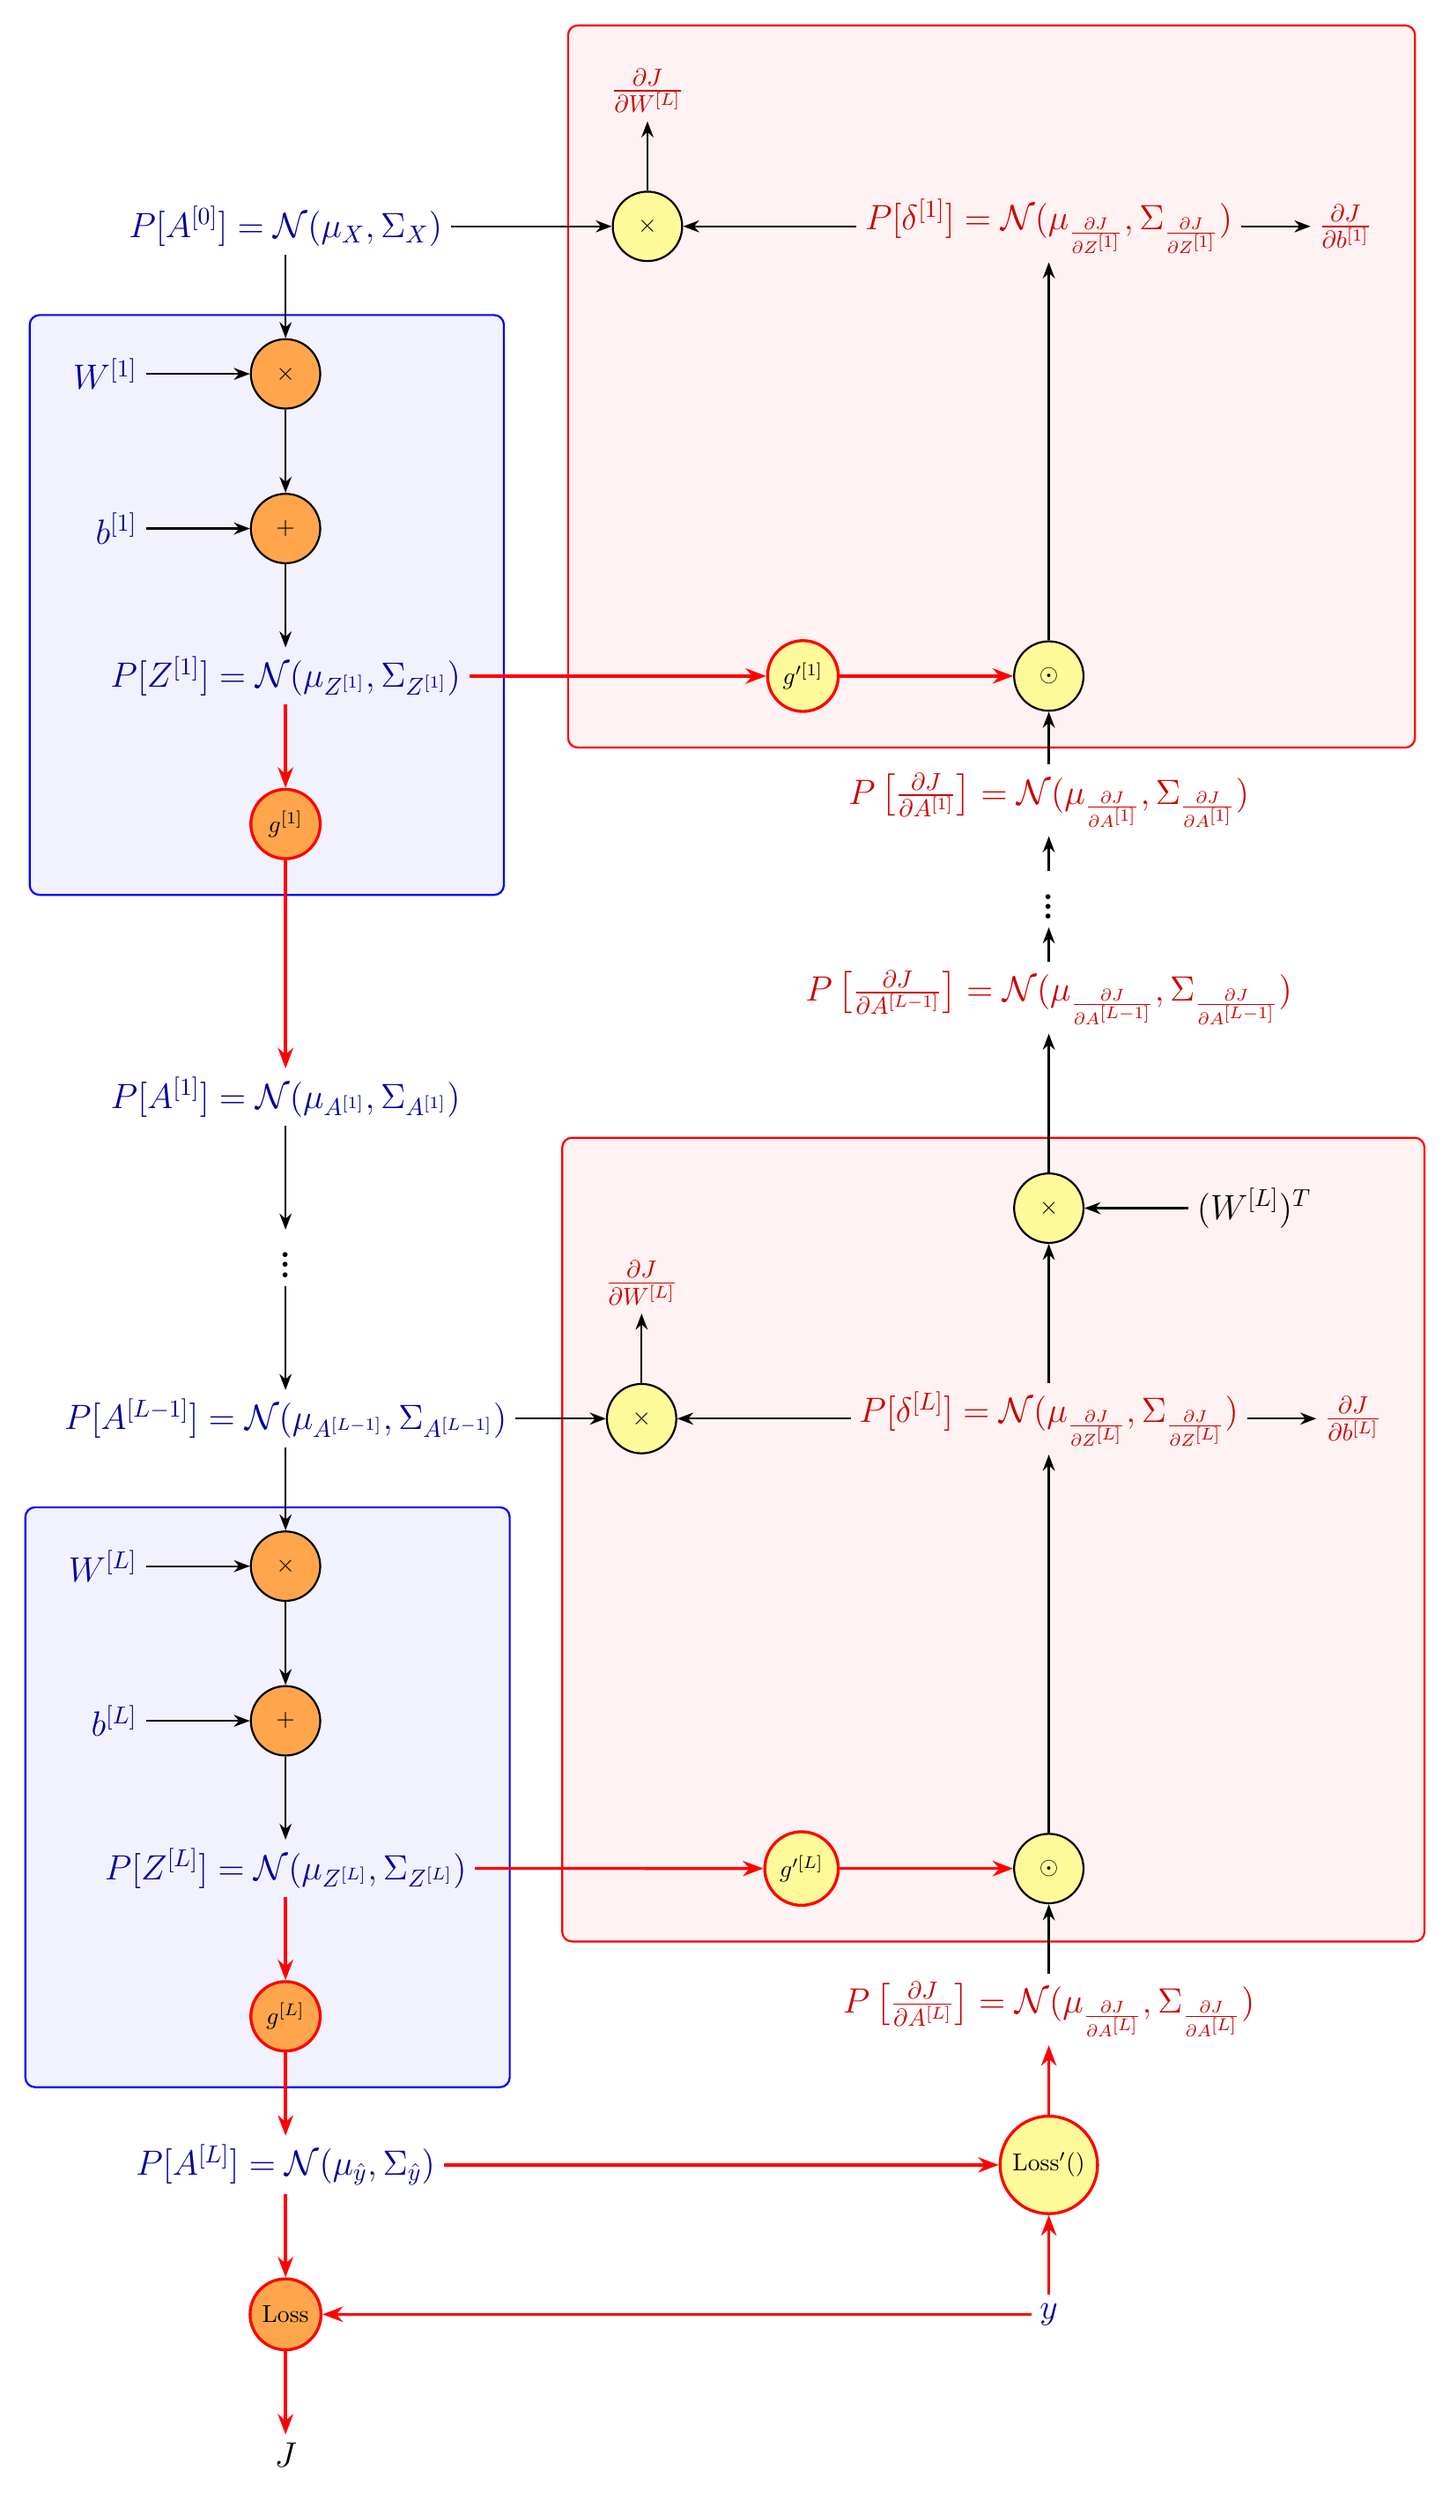
\begin{tikzpicture}[
        node distance=1.5cm and 2.5cm,
        op/.style={circle, draw, thick, minimum size=1cm, fill=yellow!40},
        fwd_op/.style={op, fill=orange!70}, % Style for forward-pass operators
        nonlinear_op/.style={draw=red, very thick}, % Style for non-linear operations
        arrow/.style={Stealth-, thick}, % Arrows flow backwards (B to A in \draw (A)--(B))
        arrow_fwd/.style={-Stealth, thick}, % Arrows for forward pass
        nonlinear_arrow_fwd/.style={arrow_fwd, red, very thick}, % Red arrows for forward non-linear
        nonlinear_arrow_back/.style={arrow, red, very thick}, % Red arrows for backward non-linear
        data/.style={font=\Large},
        grad/.style={font=\Large, text=red!80!black},
        fwd_data/.style={font=\Large, text=blue!60!black},
        layerbox/.style={draw, thick, red, rounded corners, inner sep=0.5cm, fill=red!5},
        fwd_layerbox/.style={draw, thick, blue, rounded corners, inner sep=0.5cm, fill=blue!5}
    ]
    % --- Set up layers to draw boxes in the background ---
    \pgfdeclarelayer{background}
    \pgfsetlayers{background,main}    
    
    \node[fwd_data] (A_0) {$P[A^{[0]}] = \mathcal{N}(\mu_X, \Sigma_X)$};
    \node[fwd_op, below = 1.2cm of A_0] (fwd_mult_1) {$\times$};
    \node[fwd_data, left = 1.5cm of fwd_mult_1] (W_1) {$W^{[1]}$};
    \node[fwd_op, below = 1.2cm of fwd_mult_1] (fwd_add_1) {$+$};
    \node[fwd_data, left = 1.5cm of fwd_add_1] (b_1_fwd) {$b^{[1]}$};
    \node[fwd_data, below = 1.2cm of fwd_add_1] (Z_1) {$P[Z^{[1]}] = \mathcal{N}(\mu_{Z^{[1]}}, \Sigma_{Z^{[1]}})$};

    % Connection from Z_1 to A_1
    \node[fwd_op, nonlinear_op, below = 1.2cm of Z_1] (g_1) {$g^{[1]}$};
    \node[fwd_data, below = 3cm of g_1] (A_1) {$P[A^{[1]}] = \mathcal{N}(\mu_{A^{[1]}}, \Sigma_{A^{[1]}})$};

    % Forward pass dots
    \node[font=\Huge, below = 1.5cm of A_1] (dots_fwd) {$\vdots$};  
    
    % --- Detailed Forward Pass for Layer L ---
    \node[fwd_data, below = 1.5cm of dots_fwd] (A_L_minus_1) {$P[A^{[L-1]}] = \mathcal{N}(\mu_{A^{[L-1]}}, \Sigma_{A^{[L-1]}})$};
    \node[fwd_op, below = 1.2cm of A_L_minus_1] (fwd_mult_L) {$\times$};
    \node[fwd_data, left = 1.5cm of fwd_mult_L] (W_L) {$W^{[L]}$};
    \node[fwd_op, below = 1.2cm of fwd_mult_L] (fwd_add_L) {$+$};
    \node[fwd_data, left = 1.5cm of fwd_add_L] (b_L_fwd) {$b^{[L]}$};
    \node[fwd_data, below = 1.2cm of fwd_add_L] (Z_L) {$P[Z^{[L]}] = \mathcal{N}(\mu_{Z^{[L]}}, \Sigma_{Z^{[L]}})$};
    \node[fwd_op, nonlinear_op, below = 1.2cm of Z_L] (g_L)  {$g^{[L]}$};
    \node[fwd_data, below = 1.2cm of g_L] (y_hat) {$P[A^{[L]}] = \mathcal{N}(\mu_{\hat{y}}, \Sigma_{\hat{y}})$};
    
    % --- Forward Pass Loss Calculation ---
    \node[fwd_op, nonlinear_op, below = 1.2cm of y_hat] (loss_func) {Loss};
    \node[data, below=1.2cm of loss_func] (J) {$J$};    
    
    % --- LOSS FUNCTION (AT THE BOTTOM) ----
    \node[op, nonlinear_op, right = 8cm of y_hat] (loss_prime) {Loss$'$()};    
    \node[fwd_data, at=(loss_prime.south |- loss_func.east)] (y) {$y$};

    % --- LAYER L (ABOVE LOSS) ---
    \node[grad, above = 1cm of loss_prime] (dA_L) {$P\left[\frac{\partial J}{\partial A^{[L]}}\right] = \mathcal{N}(\mu_{\frac{\partial J}{\partial A^{[L]}}}, \Sigma_{\frac{\partial J}{\partial A^{[L]}}})$};
    \node[op, above = 1cm of dA_L] (had1) {$\odot$};
    \node[op, nonlinear_op, left = 2.5cm of had1] (gprime_L_func) {$g'^{[L]}$};
    \node[grad, at=(had1.north |- A_L_minus_1.east)] (dZ_L) {$P[\delta^{[L]}] = \mathcal{N}(\mu_{\frac{\partial J}{\partial Z^{[L]}}}, \Sigma_{\frac{\partial J}{\partial Z^{[L]}}})$};

    \node[op, above = 2cm of dZ_L] (mult_a) {$\times$};
    \node[data, right = 1.5cm of mult_a] (W_L_T) {$(W^{[L]})^T$};
    \node[grad, above = 2cm of mult_a] (dA_L_minus_1) {$P\left[\frac{\partial J}{\partial A^{[L-1]}}\right] = \mathcal{N}(\mu_{\frac{\partial J}{\partial A^{[L-1]}}}, \Sigma_{\frac{\partial J}{\partial A^{[L-1]}}})$};

    \node[op, left = 2.5cm of dZ_L] (mult_w) {$\times$};
    \node[grad, above  = 1cm of mult_w] (dW_L) {$\frac{\partial J}{\partial W^{[L]}}$};
    \node[grad, right = 1cm of dZ_L] (db_L) {$\frac{\partial J}{\partial b^{[L]}}$};

    % --- CONTINUATION DOTS (ABOVE LAYER L) ---
    \node[font=\Huge, above = 0.5cm of dA_L_minus_1] (dots) {$\vdots$};

    % --- LAYER 1 (AT THE TOP) ---
    \node[grad, above = 0.5cm of dots] (dA_1) {$P\left[\frac{\partial J}{\partial A^{[1]}}\right] = \mathcal{N}(\mu_{\frac{\partial J}{\partial A^{[1]}}}, \Sigma_{\frac{\partial J}{\partial A^{[1]}}})$};
    \node[op, at=(dA_1.north |- Z_1.east)] (had_final) {$\odot$};
    \node[op, nonlinear_op, left = 2.5cm of had_final] (gprime_1_func) {$g'^{[1]}$};
    \node[grad, at=(had_final.north |- A_0.east)] (dZ_1) {$P[\delta^{[1]}] = \mathcal{N}(\mu_{\frac{\partial J}{\partial Z^{[1]}}}, \Sigma_{\frac{\partial J}{\partial Z^{[1]}}})$};

    \node[op, left = 2.5cm of dZ_1] (mult_w_final) {$\times$};
    \node[grad, above = 1cm of mult_w_final] (dW_1) {$\frac{\partial J}{\partial W^{[L]}}$};
    \node[grad, right = 1cm of dZ_1] (db_1) {$\frac{\partial J}{\partial b^{[1]}}$};

    % --- ARROWS ---
    % Forward Pass Arrows
    \draw[nonlinear_arrow_fwd] (y_hat) -- (loss_func);
    \draw[nonlinear_arrow_fwd] (y) -- (loss_func);
    \draw[nonlinear_arrow_fwd] (loss_func) -- (J);
    \draw[nonlinear_arrow_fwd] (Z_L) -- (g_L);
    \draw[nonlinear_arrow_fwd] (g_L) -- (y_hat);
    \draw[arrow_fwd] (A_L_minus_1) -- (fwd_mult_L);
    \draw[arrow_fwd] (W_L) -- (fwd_mult_L);
    \draw[arrow_fwd] (fwd_mult_L) -- (fwd_add_L);
    \draw[arrow_fwd] (b_L_fwd) -- (fwd_add_L);
    \draw[arrow_fwd] (fwd_add_L) -- (Z_L);
    \draw[arrow_fwd] (A_0) -- (fwd_mult_1);
    \draw[arrow_fwd] (W_1) -- (fwd_mult_1);
    \draw[arrow_fwd] (fwd_mult_1) -- (fwd_add_1);
    \draw[arrow_fwd] (b_1_fwd) -- (fwd_add_1);
    \draw[arrow_fwd] (fwd_add_1) -- (Z_1);
    \draw[nonlinear_arrow_fwd] (Z_1) -- (g_1);
    \draw[nonlinear_arrow_fwd] (g_1) -- (A_1);
    \draw[arrow_fwd] (A_1) -- (dots_fwd);
    \draw[arrow_fwd] (dots_fwd) -- (A_L_minus_1);

    % Backpropagation Arrows
    \draw[nonlinear_arrow_back] (loss_prime) -- (y_hat);
    \draw[nonlinear_arrow_back] (loss_prime) -- (y);
    \draw[nonlinear_arrow_back] (dA_L) -- (loss_prime);
    \draw[arrow] (had1) -- (dA_L);
    \draw[nonlinear_arrow_back] (had1) -- (gprime_L_func);
    \draw[nonlinear_arrow_back] (gprime_L_func) -- (Z_L);
    \draw[arrow] (dZ_L) -- (had1);
    \draw[arrow] (mult_w) -- (dZ_L);
    \draw[arrow] (mult_w) -- (A_L_minus_1);
    \draw[arrow] (dW_L) -- (mult_w);
    \draw[arrow] (db_L) -- (dZ_L);
    \draw[arrow] (mult_a) -- (dZ_L);
    \draw[arrow] (mult_a) -- (W_L_T);
    \draw[arrow] (dA_L_minus_1) -- (mult_a);
    \draw[arrow] (dots) -- (dA_L_minus_1);
    \draw[arrow] (dA_1) -- (dots);
    \draw[arrow] (had_final) -- (dA_1);
    \draw[nonlinear_arrow_back] (had_final) -- (gprime_1_func);
    \draw[nonlinear_arrow_back] (gprime_1_func) -- (Z_1);
    \draw[arrow] (dZ_1) -- (had_final);
    \draw[arrow] (mult_w_final) -- (dZ_1);
    \draw[arrow] (mult_w_final) -- (A_0);
    \draw[arrow] (dW_1) -- (mult_w_final);
    \draw[arrow] (db_1) -- (dZ_1);

\begin{pgfonlayer}{background}
    % Box for Layer L (Backpropagation)
    \node[layerbox,
          fit=(gprime_L_func) (had1) (dZ_L) (mult_a) (W_L_T) (dW_L) (db_L) ] {};
    % Box for Layer 1 (Backpropagation)
    \node[layerbox,
          fit=(gprime_1_func) (had_final) (dZ_1) (mult_w_final) (dW_1) (db_1)] {};
    % New box for Layer L (Forward Pass)
    \node[fwd_layerbox,
          fit=(W_L) (Z_L) (g_L)] {};
    % New box for Layer 1 (Forward Pass)
    \node[fwd_layerbox,
          fit=(W_1) (Z_1) (g_1)] {};
\end{pgfonlayer}

    \end{tikzpicture}%
}

\ifdefined\ispartofbook
  % This part is intentionally left blank when included in the main book.
  % The \newcommand is defined, and the chapter file is responsible for calling it.
\else
  % This part is for standalone compilation of the image.
  \combineddiagram 
  \end{document}
\fi
 % For standalone compilation
\fi

% This file defines the command for the combined forward/backward pass diagram.
% It can be compiled standalone or included in a larger document.

\ifdefined\ispartofbook
\else
  % --- Standalone Compilation Preamble ---
  \documentclass[tikz, border=10pt]{standalone}
  \usepackage{amsmath, amssymb} % For math symbols
  \usepackage{tikz}
  \usetikzlibrary{
    positioning,
    arrows.meta,
    fit,
    decorations.pathreplacing,
    calligraphy,
    shapes.geometric,
    shadows,
    chains,
    backgrounds
  }
  \begin{document}
\fi

% --- THE DIAGRAM COMMAND ---
\newcommand{\combineddiagram}{%
    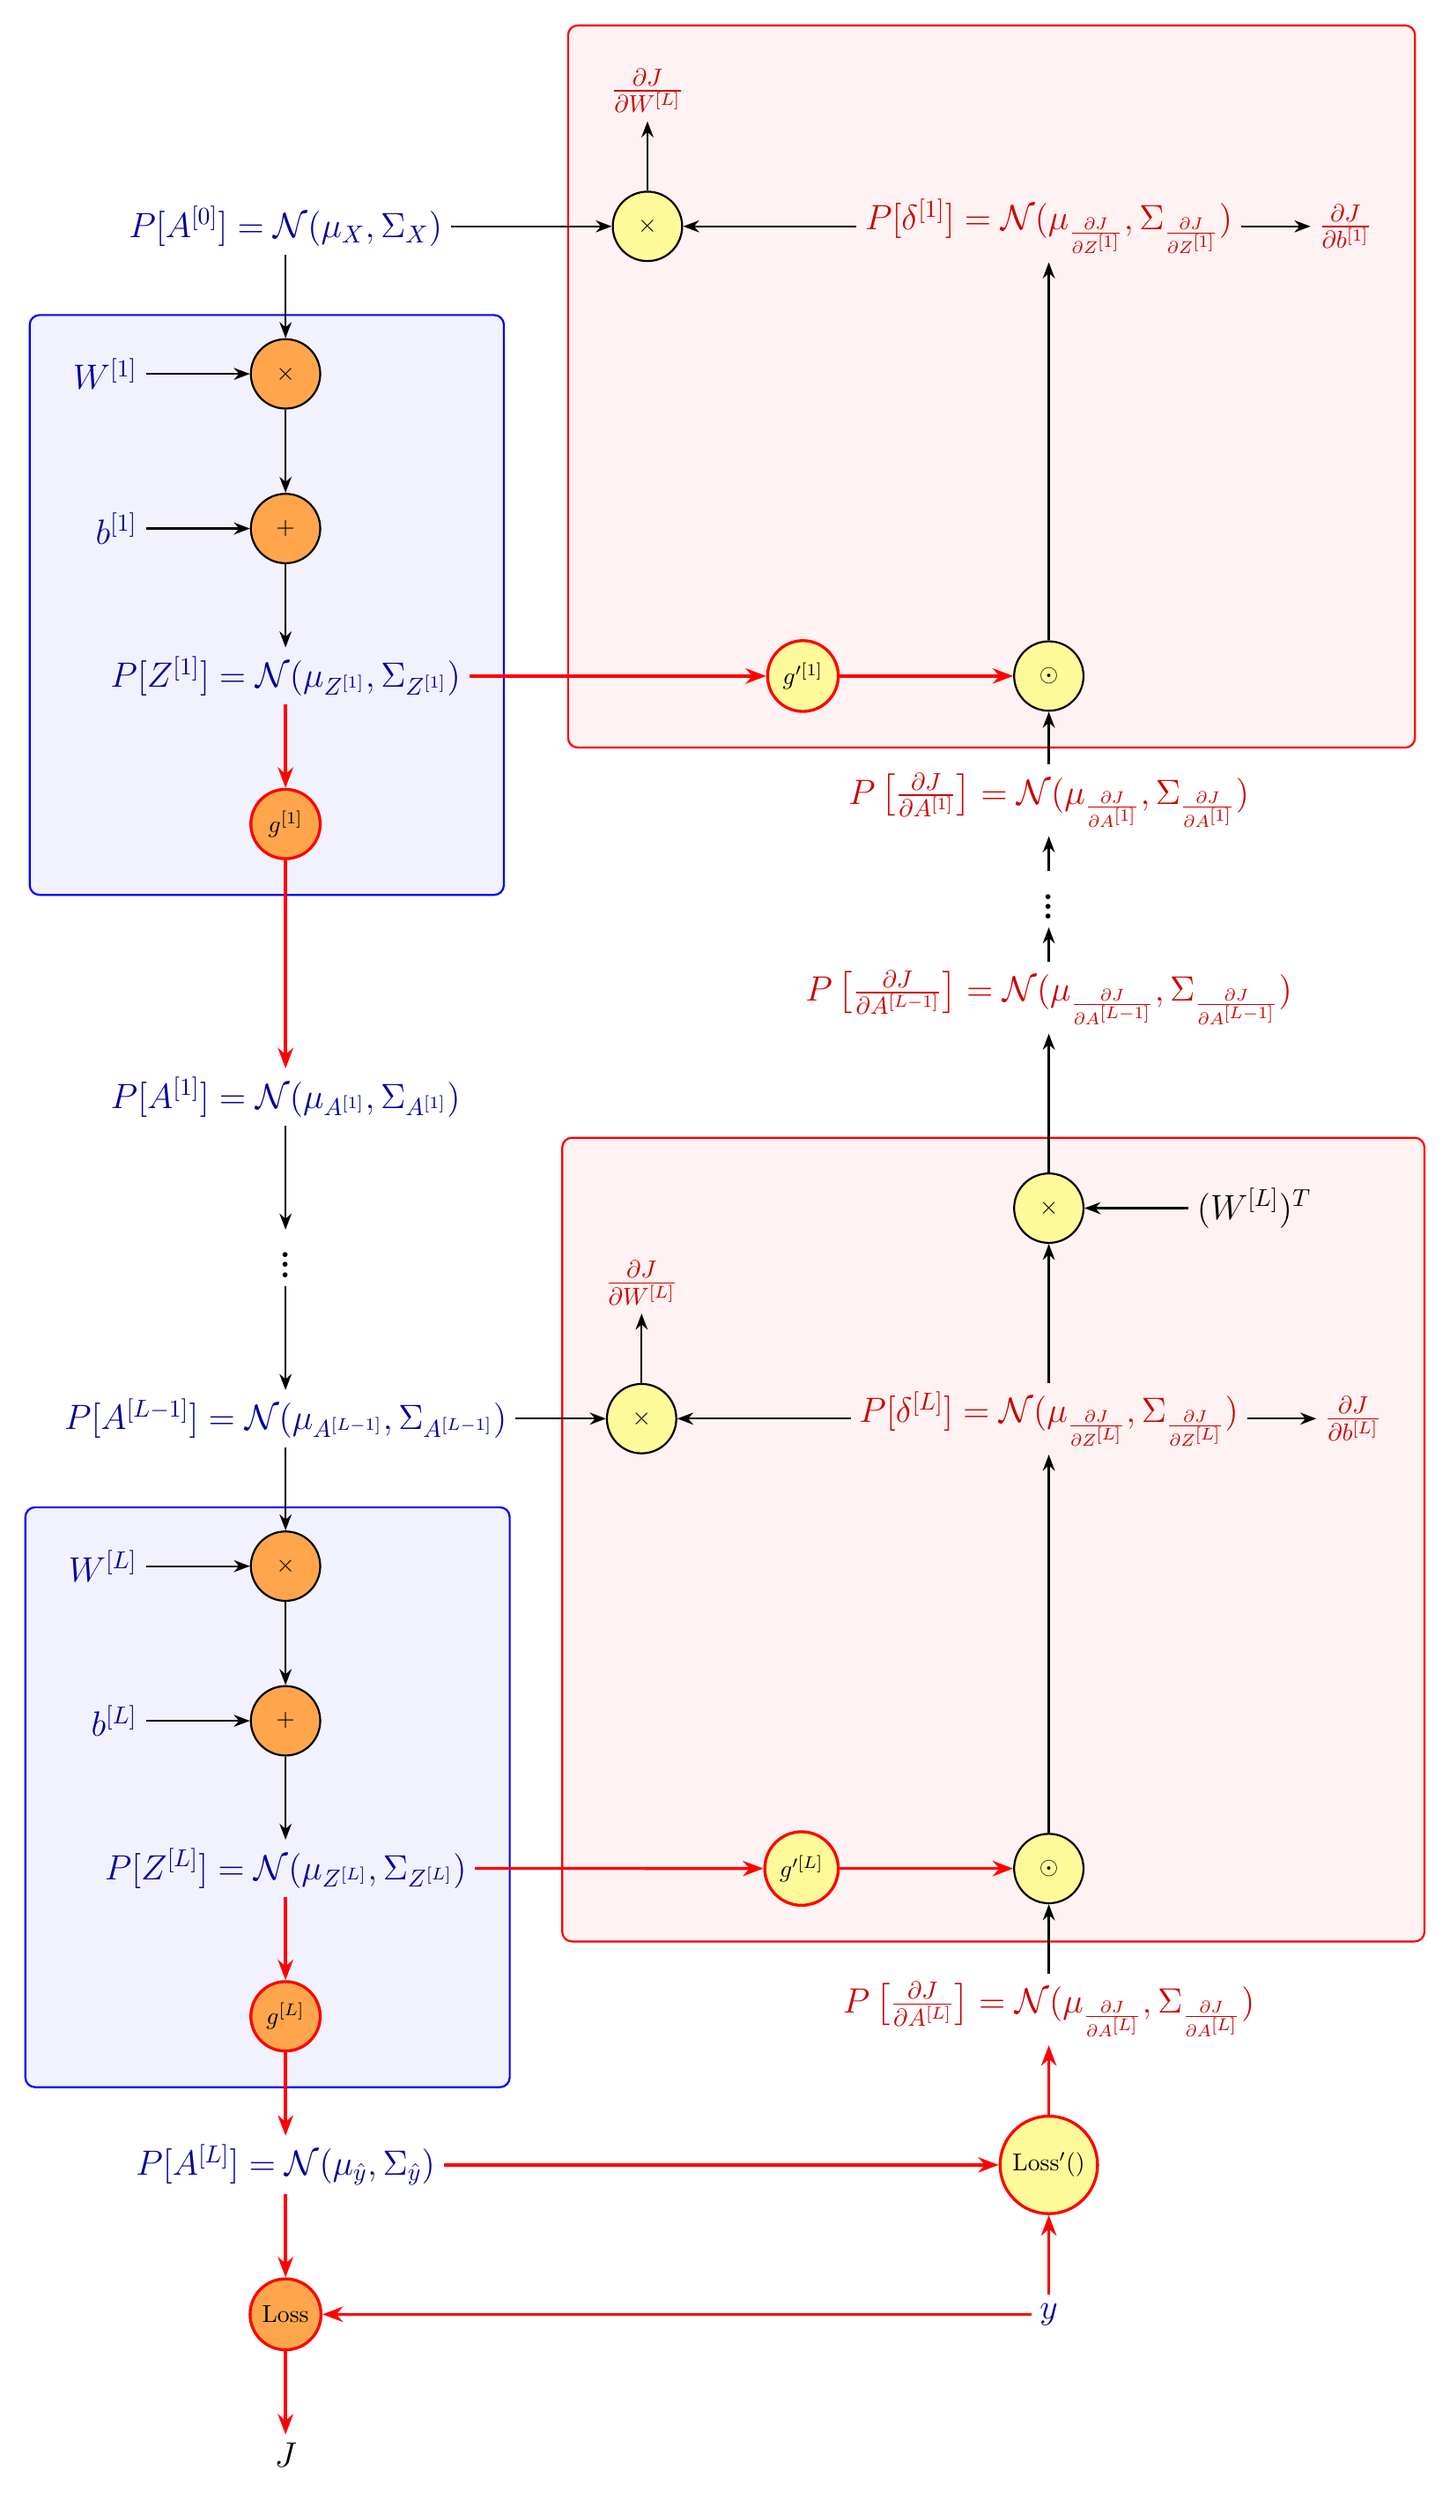
\begin{tikzpicture}[
        node distance=1.5cm and 2.5cm,
        op/.style={circle, draw, thick, minimum size=1cm, fill=yellow!40},
        fwd_op/.style={op, fill=orange!70}, % Style for forward-pass operators
        nonlinear_op/.style={draw=red, very thick}, % Style for non-linear operations
        arrow/.style={Stealth-, thick}, % Arrows flow backwards (B to A in \draw (A)--(B))
        arrow_fwd/.style={-Stealth, thick}, % Arrows for forward pass
        nonlinear_arrow_fwd/.style={arrow_fwd, red, very thick}, % Red arrows for forward non-linear
        nonlinear_arrow_back/.style={arrow, red, very thick}, % Red arrows for backward non-linear
        data/.style={font=\Large},
        grad/.style={font=\Large, text=red!80!black},
        fwd_data/.style={font=\Large, text=blue!60!black},
        layerbox/.style={draw, thick, red, rounded corners, inner sep=0.5cm, fill=red!5},
        fwd_layerbox/.style={draw, thick, blue, rounded corners, inner sep=0.5cm, fill=blue!5}
    ]
    % --- Set up layers to draw boxes in the background ---
    \pgfdeclarelayer{background}
    \pgfsetlayers{background,main}    
    
    \node[fwd_data] (A_0) {$P[A^{[0]}] = \mathcal{N}(\mu_X, \Sigma_X)$};
    \node[fwd_op, below = 1.2cm of A_0] (fwd_mult_1) {$\times$};
    \node[fwd_data, left = 1.5cm of fwd_mult_1] (W_1) {$W^{[1]}$};
    \node[fwd_op, below = 1.2cm of fwd_mult_1] (fwd_add_1) {$+$};
    \node[fwd_data, left = 1.5cm of fwd_add_1] (b_1_fwd) {$b^{[1]}$};
    \node[fwd_data, below = 1.2cm of fwd_add_1] (Z_1) {$P[Z^{[1]}] = \mathcal{N}(\mu_{Z^{[1]}}, \Sigma_{Z^{[1]}})$};

    % Connection from Z_1 to A_1
    \node[fwd_op, nonlinear_op, below = 1.2cm of Z_1] (g_1) {$g^{[1]}$};
    \node[fwd_data, below = 3cm of g_1] (A_1) {$P[A^{[1]}] = \mathcal{N}(\mu_{A^{[1]}}, \Sigma_{A^{[1]}})$};

    % Forward pass dots
    \node[font=\Huge, below = 1.5cm of A_1] (dots_fwd) {$\vdots$};  
    
    % --- Detailed Forward Pass for Layer L ---
    \node[fwd_data, below = 1.5cm of dots_fwd] (A_L_minus_1) {$P[A^{[L-1]}] = \mathcal{N}(\mu_{A^{[L-1]}}, \Sigma_{A^{[L-1]}})$};
    \node[fwd_op, below = 1.2cm of A_L_minus_1] (fwd_mult_L) {$\times$};
    \node[fwd_data, left = 1.5cm of fwd_mult_L] (W_L) {$W^{[L]}$};
    \node[fwd_op, below = 1.2cm of fwd_mult_L] (fwd_add_L) {$+$};
    \node[fwd_data, left = 1.5cm of fwd_add_L] (b_L_fwd) {$b^{[L]}$};
    \node[fwd_data, below = 1.2cm of fwd_add_L] (Z_L) {$P[Z^{[L]}] = \mathcal{N}(\mu_{Z^{[L]}}, \Sigma_{Z^{[L]}})$};
    \node[fwd_op, nonlinear_op, below = 1.2cm of Z_L] (g_L)  {$g^{[L]}$};
    \node[fwd_data, below = 1.2cm of g_L] (y_hat) {$P[A^{[L]}] = \mathcal{N}(\mu_{\hat{y}}, \Sigma_{\hat{y}})$};
    
    % --- Forward Pass Loss Calculation ---
    \node[fwd_op, nonlinear_op, below = 1.2cm of y_hat] (loss_func) {Loss};
    \node[data, below=1.2cm of loss_func] (J) {$J$};    
    
    % --- LOSS FUNCTION (AT THE BOTTOM) ----
    \node[op, nonlinear_op, right = 8cm of y_hat] (loss_prime) {Loss$'$()};    
    \node[fwd_data, at=(loss_prime.south |- loss_func.east)] (y) {$y$};

    % --- LAYER L (ABOVE LOSS) ---
    \node[grad, above = 1cm of loss_prime] (dA_L) {$P\left[\frac{\partial J}{\partial A^{[L]}}\right] = \mathcal{N}(\mu_{\frac{\partial J}{\partial A^{[L]}}}, \Sigma_{\frac{\partial J}{\partial A^{[L]}}})$};
    \node[op, above = 1cm of dA_L] (had1) {$\odot$};
    \node[op, nonlinear_op, left = 2.5cm of had1] (gprime_L_func) {$g'^{[L]}$};
    \node[grad, at=(had1.north |- A_L_minus_1.east)] (dZ_L) {$P[\delta^{[L]}] = \mathcal{N}(\mu_{\frac{\partial J}{\partial Z^{[L]}}}, \Sigma_{\frac{\partial J}{\partial Z^{[L]}}})$};

    \node[op, above = 2cm of dZ_L] (mult_a) {$\times$};
    \node[data, right = 1.5cm of mult_a] (W_L_T) {$(W^{[L]})^T$};
    \node[grad, above = 2cm of mult_a] (dA_L_minus_1) {$P\left[\frac{\partial J}{\partial A^{[L-1]}}\right] = \mathcal{N}(\mu_{\frac{\partial J}{\partial A^{[L-1]}}}, \Sigma_{\frac{\partial J}{\partial A^{[L-1]}}})$};

    \node[op, left = 2.5cm of dZ_L] (mult_w) {$\times$};
    \node[grad, above  = 1cm of mult_w] (dW_L) {$\frac{\partial J}{\partial W^{[L]}}$};
    \node[grad, right = 1cm of dZ_L] (db_L) {$\frac{\partial J}{\partial b^{[L]}}$};

    % --- CONTINUATION DOTS (ABOVE LAYER L) ---
    \node[font=\Huge, above = 0.5cm of dA_L_minus_1] (dots) {$\vdots$};

    % --- LAYER 1 (AT THE TOP) ---
    \node[grad, above = 0.5cm of dots] (dA_1) {$P\left[\frac{\partial J}{\partial A^{[1]}}\right] = \mathcal{N}(\mu_{\frac{\partial J}{\partial A^{[1]}}}, \Sigma_{\frac{\partial J}{\partial A^{[1]}}})$};
    \node[op, at=(dA_1.north |- Z_1.east)] (had_final) {$\odot$};
    \node[op, nonlinear_op, left = 2.5cm of had_final] (gprime_1_func) {$g'^{[1]}$};
    \node[grad, at=(had_final.north |- A_0.east)] (dZ_1) {$P[\delta^{[1]}] = \mathcal{N}(\mu_{\frac{\partial J}{\partial Z^{[1]}}}, \Sigma_{\frac{\partial J}{\partial Z^{[1]}}})$};

    \node[op, left = 2.5cm of dZ_1] (mult_w_final) {$\times$};
    \node[grad, above = 1cm of mult_w_final] (dW_1) {$\frac{\partial J}{\partial W^{[L]}}$};
    \node[grad, right = 1cm of dZ_1] (db_1) {$\frac{\partial J}{\partial b^{[1]}}$};

    % --- ARROWS ---
    % Forward Pass Arrows
    \draw[nonlinear_arrow_fwd] (y_hat) -- (loss_func);
    \draw[nonlinear_arrow_fwd] (y) -- (loss_func);
    \draw[nonlinear_arrow_fwd] (loss_func) -- (J);
    \draw[nonlinear_arrow_fwd] (Z_L) -- (g_L);
    \draw[nonlinear_arrow_fwd] (g_L) -- (y_hat);
    \draw[arrow_fwd] (A_L_minus_1) -- (fwd_mult_L);
    \draw[arrow_fwd] (W_L) -- (fwd_mult_L);
    \draw[arrow_fwd] (fwd_mult_L) -- (fwd_add_L);
    \draw[arrow_fwd] (b_L_fwd) -- (fwd_add_L);
    \draw[arrow_fwd] (fwd_add_L) -- (Z_L);
    \draw[arrow_fwd] (A_0) -- (fwd_mult_1);
    \draw[arrow_fwd] (W_1) -- (fwd_mult_1);
    \draw[arrow_fwd] (fwd_mult_1) -- (fwd_add_1);
    \draw[arrow_fwd] (b_1_fwd) -- (fwd_add_1);
    \draw[arrow_fwd] (fwd_add_1) -- (Z_1);
    \draw[nonlinear_arrow_fwd] (Z_1) -- (g_1);
    \draw[nonlinear_arrow_fwd] (g_1) -- (A_1);
    \draw[arrow_fwd] (A_1) -- (dots_fwd);
    \draw[arrow_fwd] (dots_fwd) -- (A_L_minus_1);

    % Backpropagation Arrows
    \draw[nonlinear_arrow_back] (loss_prime) -- (y_hat);
    \draw[nonlinear_arrow_back] (loss_prime) -- (y);
    \draw[nonlinear_arrow_back] (dA_L) -- (loss_prime);
    \draw[arrow] (had1) -- (dA_L);
    \draw[nonlinear_arrow_back] (had1) -- (gprime_L_func);
    \draw[nonlinear_arrow_back] (gprime_L_func) -- (Z_L);
    \draw[arrow] (dZ_L) -- (had1);
    \draw[arrow] (mult_w) -- (dZ_L);
    \draw[arrow] (mult_w) -- (A_L_minus_1);
    \draw[arrow] (dW_L) -- (mult_w);
    \draw[arrow] (db_L) -- (dZ_L);
    \draw[arrow] (mult_a) -- (dZ_L);
    \draw[arrow] (mult_a) -- (W_L_T);
    \draw[arrow] (dA_L_minus_1) -- (mult_a);
    \draw[arrow] (dots) -- (dA_L_minus_1);
    \draw[arrow] (dA_1) -- (dots);
    \draw[arrow] (had_final) -- (dA_1);
    \draw[nonlinear_arrow_back] (had_final) -- (gprime_1_func);
    \draw[nonlinear_arrow_back] (gprime_1_func) -- (Z_1);
    \draw[arrow] (dZ_1) -- (had_final);
    \draw[arrow] (mult_w_final) -- (dZ_1);
    \draw[arrow] (mult_w_final) -- (A_0);
    \draw[arrow] (dW_1) -- (mult_w_final);
    \draw[arrow] (db_1) -- (dZ_1);

\begin{pgfonlayer}{background}
    % Box for Layer L (Backpropagation)
    \node[layerbox,
          fit=(gprime_L_func) (had1) (dZ_L) (mult_a) (W_L_T) (dW_L) (db_L) ] {};
    % Box for Layer 1 (Backpropagation)
    \node[layerbox,
          fit=(gprime_1_func) (had_final) (dZ_1) (mult_w_final) (dW_1) (db_1)] {};
    % New box for Layer L (Forward Pass)
    \node[fwd_layerbox,
          fit=(W_L) (Z_L) (g_L)] {};
    % New box for Layer 1 (Forward Pass)
    \node[fwd_layerbox,
          fit=(W_1) (Z_1) (g_1)] {};
\end{pgfonlayer}

    \end{tikzpicture}%
}

\ifdefined\ispartofbook
  % This part is intentionally left blank when included in the main book.
  % The \newcommand is defined, and the chapter file is responsible for calling it.
\else
  % This part is for standalone compilation of the image.
  \combineddiagram 
  \end{document}
\fi
 % Include the new diagram command file

\section{A Conceptual Framework for Statistical Propagation}
\label{sec:conceptual_framework_stats}

In Chapter \ref{chap:propagation}, we detailed the mechanics of how a neural network learns from data. The process, as illustrated in Figure \ref{fig:combine}, follows a clear path: a batch of data points, $\matr{X}$, is fed forward through the network, a scalar loss is computed based on the difference between the prediction and the true label, and the gradient of this loss is propagated backward to update the network's parameters. This paradigm, known as Stochastic Gradient Descent (SGD), has been the engine of the deep learning revolution. It is, however, fundamentally a sample-based process. The network learns by incrementally correcting its errors on small, discrete subsets of the data, iteratively adjusting its weights to better fit the training set.

This subchapter proposes a conceptual departure from this paradigm. We will explore the author's intention to reframe the learning process not as an operation on discrete data points, but as a holistic transformation of entire probability distributions. This shift in perspective is the foundation of a powerful set of analytical tools that allow us to understand network behavior in a more deterministic and principled way, moving from a stochastic approximation of the learning process to an analytical characterization of it.

\subsection{From Data Points to Distributions}
Let us re-examine the propagation diagram (Figure \ref{fig:combine}) through a new, statistical lens. Instead of viewing the input $\matr{X}$ as a matrix of $m$ data samples, we will now posit that the entire input dataset can be effectively modeled by a single, high-dimensional Multivariate Normal distribution, $\mathcal{N}(\boldsymbol{\mu}_X, \boldsymbol{\Sigma}_X)$. The mean vector $\boldsymbol{\mu}_X$ represents the "average" input, and the covariance matrix $\boldsymbol{\Sigma}_X$ captures the variance of each feature and the correlations between them across the entire dataset.

Under this new interpretation, the very nature of the information flowing through the network changes, as illustrated in Figure \ref{fig:stat_prop_diagram}.

\begin{figure}[h!]
    \centering
    \scalebox{0.6}{\statisticalpropagationdiagram}
    \caption{A conceptual comparison between standard sample-based propagation (top) and the proposed holistic, distribution-based propagation (bottom). Instead of processing a batch of data to get a scalar loss, the network transforms an entire input distribution to an output distribution, and the "loss" becomes a measure of divergence between distributions.}
    \label{fig:stat_prop_diagram}
\end{figure}

The forward pass is transformed from a data processing pipeline into a \textbf{distributional transformation pipeline}. Its purpose is to compute how the network warps the input distribution into an output distribution.
\begin{itemize}
    \item The input, $A^{[0]}$, is no longer a matrix of data points, but the parameters $(\boldsymbol{\mu}_X, \boldsymbol{\Sigma}_X)$ that define the input statistical manifold.
    \item Each subsequent activation, $A^{[l]}$, is also not a set of vectors, but a new probability distribution with its own mean and covariance, $(\boldsymbol{\mu}_{A^{[l]}}, \boldsymbol{\Sigma}_{A^{[l]}})$.
\end{itemize}

\subsection{Re-interpreting the Backward Pass}
This conceptual shift extends naturally to the backward pass. In the standard paradigm, the loss $J$ is a scalar value representing the error for a specific mini-batch. In our new framework, the loss must be a measure of the dissimilarity between two entire probability distributions: the network's final output distribution and a target distribution (e.g., the distribution of the true labels). This could be a metric like the Kullback-Leibler (KL) divergence or the Wasserstein distance.

Consequently, the backward pass undergoes a similar transformation:
\begin{itemize}
    \item It no longer propagates the gradient of a scalar loss. Instead, it must propagate the "gradient" of this distributional divergence.
    \item The error signals, $\delta^{[l]}$, are no longer vectors of error values for each sample in a batch. They are themselves distributions, characterized by a mean and covariance, representing the statistical properties of the error signal.
    \item The ultimate goal of this "statistical backpropagation" is to determine how to update the network's weights to optimally transform the input distribution into the target distribution, minimizing the divergence between them.
\end{itemize}

\subsection{The Recursive Challenge of Non-Linearity}
The ultimate goal of this forward distributional pass is to determine the statistical properties of the final pre-activations, $p(\vect{Z}^{[L]})$, as this distribution directly informs the network's final output. However, one cannot simply jump from the input distribution $p(\vect{X})$ to the final pre-activation distribution $p(\vect{Z}^{[L]})$. The presence of non-linear activation functions makes this a recursive, layer-by-layer challenge.

To find the distribution at the end of the network, we must be able to solve a fundamental, recurring problem at each layer: given an input distribution, what is the output distribution after it has been transformed by both a linear operation and a non-linear one? Specifically, the process is as follows:
\begin{enumerate}
    \item The input distribution to a layer, $p(\vect{A}^{[l-1]})$, is first passed through the affine transformation to produce the pre-activation distribution, $p(\vect{Z}^{[l]})$.
    \item This pre-activation distribution is then passed through the element-wise non-linear ReLU function, producing the post-activation distribution, $p(\vect{A}^{[l]})$.
    \item This new distribution, $p(\vect{A}^{[l]})$, then becomes the input for the next layer, and the process repeats.
\end{enumerate}
This chain of transformations—where the output distribution of one layer becomes the input distribution for the next—is the essence of \textbf{Analytical Moment Propagation (AMP)} \cite{Wright2024AnalyticCovariance, Schoenholz2017DeepInfoProp}. The core analytical task is to derive the mathematical rules that govern how the moments (mean and covariance) of a distribution are altered by each of these linear and non-linear steps.

This subchapter has laid out the conceptual vision. The following subchapters will provide the detailed mathematical derivations required to turn this vision into a concrete analytical framework for both the forward and backward passes.

\ifdefined\ispartofbook
\else
  \end{document}
\fi

\ifdefined\ispartofbook
\else
  % Preamble for "A Journey into Deep Learning"

% --- DOCUMENT CLASS & GEOMETRY ---
\documentclass[11pt, a4paper]{report} % Changed from 'article' to 'report' to enable \chapter command
\usepackage[margin=1in]{geometry} % Set page margins

% --- FONT & ENCODING ---
\usepackage[T1]{fontenc}
\usepackage[utf8]{inputenc}

% --- MATHEMATICS & SYMBOLS ---
\usepackage{amsmath, amssymb, amsthm} % For advanced math typesetting and theorems
\usepackage{amsfonts}                 % For math fonts
\usepackage{bm}                       % For bold math symbols

% --- GRAPHICS & TABLES ---
\usepackage{graphicx}                 % To include graphics
\usepackage{booktabs}                 % For professional-quality tables
\usepackage{caption}                  % For customizing captions

% --- LISTS & LAYOUT ---
\usepackage{enumitem}                 % For list customization
\usepackage{cases}                    % For cases environment

% --- TIKZ GRAPHICS PACKAGES (NEWLY ADDED) ---
\usepackage{tikz}
\usetikzlibrary{
    positioning,
    arrows.meta,
    fit,
    decorations.pathreplacing,
    calligraphy,
    shapes.geometric,
    shadows,
    chains,
    backgrounds % For layering
}

% --- HYPERLINKS & URLS ---
\usepackage[hyphens]{url}             % For URL formatting
\usepackage{hyperref}                 % For hyperlinks and cross-references
\hypersetup{
    colorlinks=true,
    linkcolor=blue,
    filecolor=magenta,
    urlcolor=cyan,
    citecolor=red,
}

% --- CUSTOM COMMANDS ---
\newcommand{\vect}[1]{\mathbf{#1}}
\newcommand{\matr}[1]{\mathbf{#1}}
\newcommand{\normdist}{\mathcal{N}}
\newcommand{\reals}{\mathbb{R}}
\newcommand{\E}{\mathbb{E}}

  \begin{document}
  % This file defines the command for illustrating AMP through a single layer.
% It can be compiled standalone or included in a larger document.

\ifdefined\ispartofbook
\else
  % --- Standalone Compilation Preamble ---
  \documentclass[tikz, border=10pt]{standalone}
  \usepackage{tikz}
  \usetikzlibrary{arrows.meta, positioning}
  \usepackage{amsmath, amssymb} % Added for \vect command
  \newcommand{\vect}[1]{\mathbf{#1}} % Added for \vect command
  \begin{document}
\fi

% --- THE DIAGRAM COMMAND ---
\newcommand{\amplayerdiagram}{%
    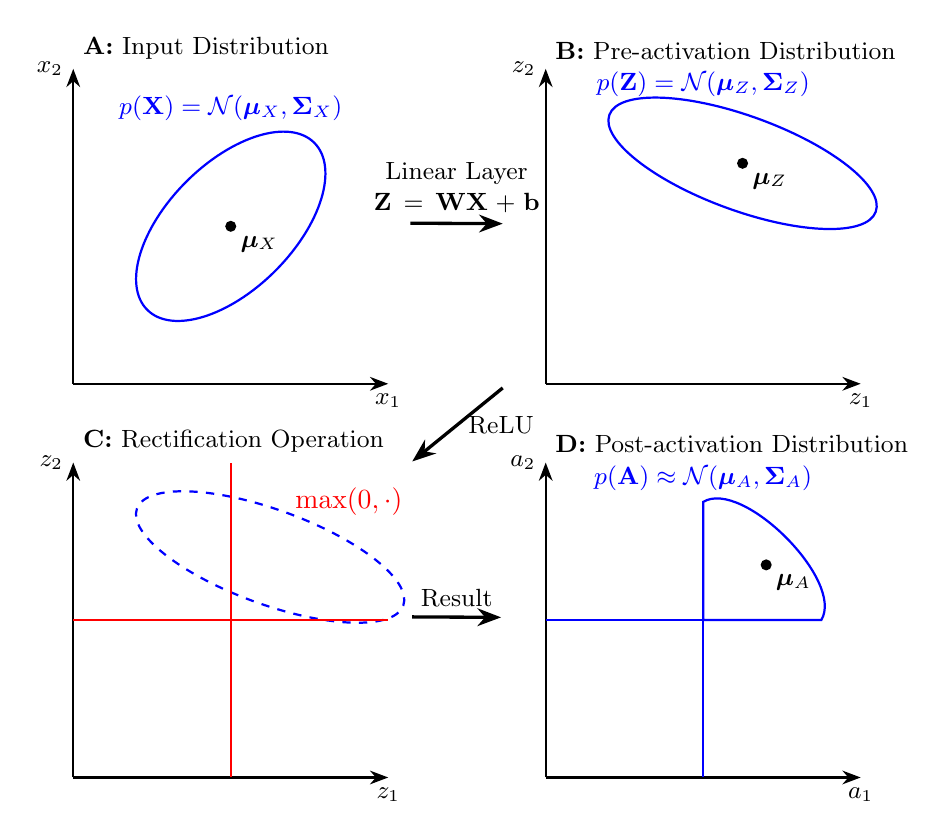
\begin{tikzpicture}[
        font=\sffamily,
        every node/.style={font=\small, align=center}
    ]
    % --- Panel A: Input Distribution ---
    \begin{scope}[local bounding box=panelA]
        \draw[-Stealth, thick] (-2,-2) -- (2,-2) node[below] {$x_1$};
        \draw[-Stealth, thick] (-2,-2) -- (-2,2) node[left] {$x_2$};
        \node[above right] at (-2,2) {\textbf{A:} Input Distribution};
        \draw[blue, thick, rotate around={45:(0,0)}] (0,0) ellipse (1.5cm and 0.8cm);
        \fill[black] (0,0) circle (2pt) node[below right] {$\boldsymbol{\mu}_X$};
        \node[blue] at (0, 1.5) {$p(\vect{X}) = \mathcal{N}(\boldsymbol{\mu}_X, \boldsymbol{\Sigma}_X)$};
    \end{scope}

    % --- Panel B: Linear Transformation ---
    \begin{scope}[local bounding box=panelB, xshift=6cm]
        \draw[-Stealth, thick] (-2,-2) -- (2,-2) node[below] {$z_1$};
        \draw[-Stealth, thick] (-2,-2) -- (-2,2) node[left] {$z_2$};
        \node[above right] at (-2,2) {\textbf{B:} Pre-activation Distribution};
        \draw[blue, thick, rotate around={-20:(0.5,0.8)}] (0.5,0.8) ellipse (1.8cm and 0.6cm);
        \fill[black] (0.5,0.8) circle (2pt) node[below right] {$\boldsymbol{\mu}_Z$};
        \node[blue] at (0, 1.8) {$p(\vect{Z}) = \mathcal{N}(\boldsymbol{\mu}_Z, \boldsymbol{\Sigma}_Z)$};
    \end{scope}

    % --- Panel C: Non-Linear Rectification ---
    \begin{scope}[local bounding box=panelC, yshift=-5cm]
        \draw[-Stealth, thick] (-2,-2) -- (2,-2) node[below] {$z_1$};
        \draw[-Stealth, thick] (-2,-2) -- (-2,2) node[left] {$z_2$};
        \node[above right] at (-2,2) {\textbf{C:} Rectification Operation};
        % Draw original ellipse for context
        \draw[blue, thick, dashed, rotate around={-20:(0.5,0.8)}] (0.5,0.8) ellipse (1.8cm and 0.6cm);
        % Draw axes for rectification
        \draw[red, thick] (-2,0) -- (2,0);
        \draw[red, thick] (0,-2) -- (0,2);
        \node[red, font=\bfseries] at (1.5, 1.5) {$\max(0, \cdot)$};
    \end{scope}

    % --- Panel D: Output Distribution (MODIFIED FOR ALIGNMENT) ---
    \begin{scope}[local bounding box=panelD, xshift=6cm, yshift=-5cm]
        \draw[-Stealth, thick] (-2,-2) -- (2,-2) node[below] {$a_1$};
        \draw[-Stealth, thick] (-2,-2) -- (-2,2) node[left] {$a_2$};
        \node[above right] at (-2,2) {\textbf{D:} Post-activation Distribution};
        % Draw an approximate shape for the rectified distribution, now centered
        \draw[blue, thick] (0,-2) -- (0,0) -- (-2,0); % Boundary axes
        \draw[blue, thick] (0,0) -- (0,1.5) .. controls (0.5,1.8) and (1.8,0.5) .. (1.5,0) -- (0,0);
        \fill[black] (0.8,0.7) circle (2pt) node[below right] {$\boldsymbol{\mu}_A$};
        \node[blue] at (0, 1.8) {$p(\vect{A}) \approx \mathcal{N}(\boldsymbol{\mu}_A, \boldsymbol{\Sigma}_A)$};
    \end{scope}

    % --- Arrows connecting panels ---
    \draw[-{Stealth[length=3mm]}, very thick] (panelA) -- (panelB) node[midway, above, text width=3cm] {Linear Layer \\ $\vect{Z} = \vect{W}\vect{X} + \vect{b}$};
    \draw[-{Stealth[length=3mm]}, very thick] (panelB) -- (panelC) node[midway, right] {ReLU};
    \draw[-{Stealth[length=3mm]}, very thick] (panelC) -- (panelD) node[midway, above] {Result};

    \end{tikzpicture}%
}

\ifdefined\ispartofbook
  % This part is intentionally left blank when included in the main book.
\else
  % This part is for standalone compilation of the image.
  \amplayerdiagram
  \end{document}
\fi
 % For standalone compilation
\fi

% This file defines the command for illustrating AMP through a single layer.
% It can be compiled standalone or included in a larger document.

\ifdefined\ispartofbook
\else
  % --- Standalone Compilation Preamble ---
  \documentclass[tikz, border=10pt]{standalone}
  \usepackage{tikz}
  \usetikzlibrary{arrows.meta, positioning}
  \usepackage{amsmath, amssymb} % Added for \vect command
  \newcommand{\vect}[1]{\mathbf{#1}} % Added for \vect command
  \begin{document}
\fi

% --- THE DIAGRAM COMMAND ---
\newcommand{\amplayerdiagram}{%
    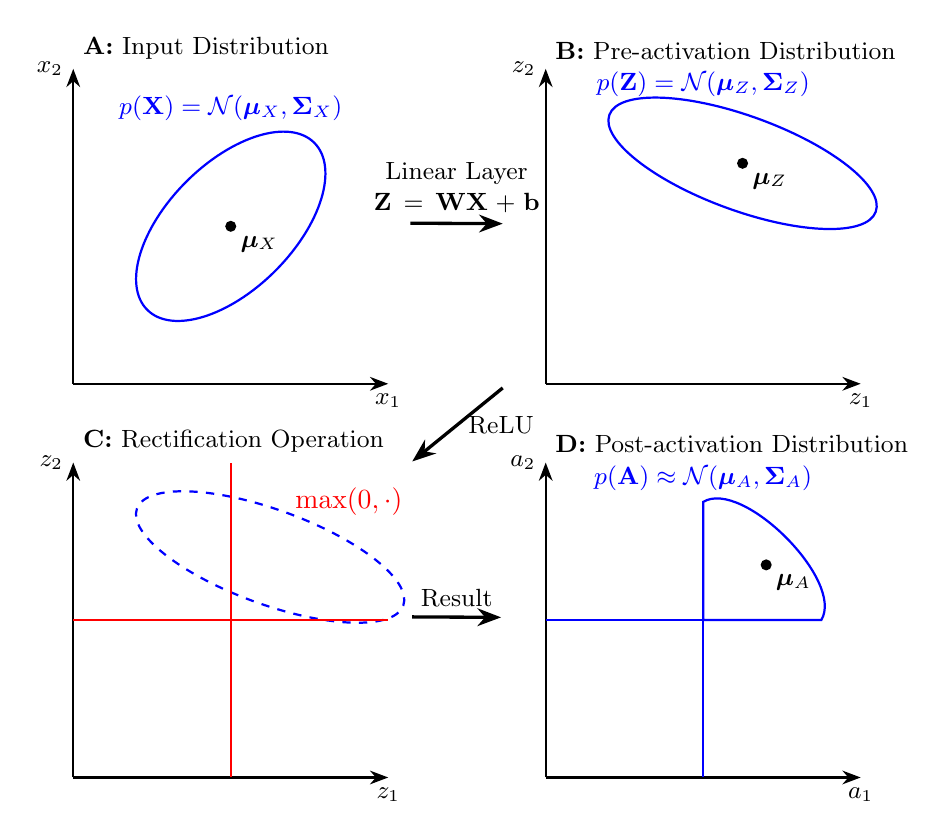
\begin{tikzpicture}[
        font=\sffamily,
        every node/.style={font=\small, align=center}
    ]
    % --- Panel A: Input Distribution ---
    \begin{scope}[local bounding box=panelA]
        \draw[-Stealth, thick] (-2,-2) -- (2,-2) node[below] {$x_1$};
        \draw[-Stealth, thick] (-2,-2) -- (-2,2) node[left] {$x_2$};
        \node[above right] at (-2,2) {\textbf{A:} Input Distribution};
        \draw[blue, thick, rotate around={45:(0,0)}] (0,0) ellipse (1.5cm and 0.8cm);
        \fill[black] (0,0) circle (2pt) node[below right] {$\boldsymbol{\mu}_X$};
        \node[blue] at (0, 1.5) {$p(\vect{X}) = \mathcal{N}(\boldsymbol{\mu}_X, \boldsymbol{\Sigma}_X)$};
    \end{scope}

    % --- Panel B: Linear Transformation ---
    \begin{scope}[local bounding box=panelB, xshift=6cm]
        \draw[-Stealth, thick] (-2,-2) -- (2,-2) node[below] {$z_1$};
        \draw[-Stealth, thick] (-2,-2) -- (-2,2) node[left] {$z_2$};
        \node[above right] at (-2,2) {\textbf{B:} Pre-activation Distribution};
        \draw[blue, thick, rotate around={-20:(0.5,0.8)}] (0.5,0.8) ellipse (1.8cm and 0.6cm);
        \fill[black] (0.5,0.8) circle (2pt) node[below right] {$\boldsymbol{\mu}_Z$};
        \node[blue] at (0, 1.8) {$p(\vect{Z}) = \mathcal{N}(\boldsymbol{\mu}_Z, \boldsymbol{\Sigma}_Z)$};
    \end{scope}

    % --- Panel C: Non-Linear Rectification ---
    \begin{scope}[local bounding box=panelC, yshift=-5cm]
        \draw[-Stealth, thick] (-2,-2) -- (2,-2) node[below] {$z_1$};
        \draw[-Stealth, thick] (-2,-2) -- (-2,2) node[left] {$z_2$};
        \node[above right] at (-2,2) {\textbf{C:} Rectification Operation};
        % Draw original ellipse for context
        \draw[blue, thick, dashed, rotate around={-20:(0.5,0.8)}] (0.5,0.8) ellipse (1.8cm and 0.6cm);
        % Draw axes for rectification
        \draw[red, thick] (-2,0) -- (2,0);
        \draw[red, thick] (0,-2) -- (0,2);
        \node[red, font=\bfseries] at (1.5, 1.5) {$\max(0, \cdot)$};
    \end{scope}

    % --- Panel D: Output Distribution (MODIFIED FOR ALIGNMENT) ---
    \begin{scope}[local bounding box=panelD, xshift=6cm, yshift=-5cm]
        \draw[-Stealth, thick] (-2,-2) -- (2,-2) node[below] {$a_1$};
        \draw[-Stealth, thick] (-2,-2) -- (-2,2) node[left] {$a_2$};
        \node[above right] at (-2,2) {\textbf{D:} Post-activation Distribution};
        % Draw an approximate shape for the rectified distribution, now centered
        \draw[blue, thick] (0,-2) -- (0,0) -- (-2,0); % Boundary axes
        \draw[blue, thick] (0,0) -- (0,1.5) .. controls (0.5,1.8) and (1.8,0.5) .. (1.5,0) -- (0,0);
        \fill[black] (0.8,0.7) circle (2pt) node[below right] {$\boldsymbol{\mu}_A$};
        \node[blue] at (0, 1.8) {$p(\vect{A}) \approx \mathcal{N}(\boldsymbol{\mu}_A, \boldsymbol{\Sigma}_A)$};
    \end{scope}

    % --- Arrows connecting panels ---
    \draw[-{Stealth[length=3mm]}, very thick] (panelA) -- (panelB) node[midway, above, text width=3cm] {Linear Layer \\ $\vect{Z} = \vect{W}\vect{X} + \vect{b}$};
    \draw[-{Stealth[length=3mm]}, very thick] (panelB) -- (panelC) node[midway, right] {ReLU};
    \draw[-{Stealth[length=3mm]}, very thick] (panelC) -- (panelD) node[midway, above] {Result};

    \end{tikzpicture}%
}

\ifdefined\ispartofbook
  % This part is intentionally left blank when included in the main book.
\else
  % This part is for standalone compilation of the image.
  \amplayerdiagram
  \end{document}
\fi
 % Include the AMP Layer diagram command file

\section{The Forward Pass on a Distribution}
\label{sec:forward_pass_distribution}

This subchapter provides the detailed mathematical derivations for the concepts introduced in Subchapter 7.1. We will explain how to analytically propagate the first two statistical moments—the mean vector and the covariance matrix—through a single, complete neural network layer. This process, known as Analytical Moment Propagation (AMP), involves two distinct steps: propagation through the layer's linear (affine) transformation and propagation through its non-linear activation function.

\subsection{Step 1: Propagation through the Linear Layer}
Let the input to a layer be an $N$-dimensional random vector $\vect{X}$ that follows a multivariate normal distribution, $\vect{X} \sim \mathcal{N}(\boldsymbol{\mu}_X, \boldsymbol{\Sigma}_X)$. The first operation in a standard dense layer is the affine transformation to compute the pre-activation vector $\vect{Z}$:
\begin{equation}
    \vect{Z} = \vect{W}\vect{X} + \vect{b}
\end{equation}
where $\vect{W}$ is the weight matrix and $\vect{b}$ is the bias vector.

Because the multivariate normal distribution is closed under affine transformations, the resulting pre-activation vector $\vect{Z}$ is also exactly normally distributed. We can find its mean and covariance using the standard rules for linear transformations of random vectors:
\begin{itemize}
    \item \textbf{The new mean vector, $\boldsymbol{\mu}_Z$,} is found by applying the transformation to the original mean:
    \begin{equation}
        \boldsymbol{\mu}_Z = \E[\vect{W}\vect{X} + \vect{b}] = \vect{W}\E[\vect{X}] + \vect{b} = \vect{W}\boldsymbol{\mu}_X + \vect{b}
    \end{equation}
    \item \textbf{The new covariance matrix, $\boldsymbol{\Sigma}_Z$,} is found by transforming the original covariance:
    \begin{equation}
        \boldsymbol{\Sigma}_Z = \text{Cov}(\vect{W}\vect{X} + \vect{b}) = \vect{W}\text{Cov}(\vect{X})\vect{W}^T = \vect{W}\boldsymbol{\Sigma}_X\vect{W}^T
    \end{equation}
\end{itemize}
This first step is analytically exact and straightforward. It transforms the input Gaussian distribution into a new Gaussian distribution that has been rotated, scaled, and shifted in the vector space.

\subsection{Step 2: Propagation through the Non-Linear (ReLU) Layer}
The second step presents the core analytical challenge. The pre-activation vector $\vect{Z} \sim \mathcal{N}(\boldsymbol{\mu}_Z, \boldsymbol{\Sigma}_Z)$ is passed through the element-wise ReLU activation function to produce the post-activation vector $\vect{A}$:
\begin{equation}
    \vect{A} = \max(\vect{0}, \vect{Z})
\end{equation}
The resulting distribution, $p(\vect{A})$, is a Rectified Multivariate Normal (RMVN) distribution, which is no longer Gaussian. As discussed in Chapter \ref{chap:multivariate_stats}, its moments are analytically intractable for high dimensions. Therefore, AMP proceeds by computing the exact first two moments of this non-Gaussian distribution.

The mean and variance of each component $A_i$ can be computed independently using the univariate rectified Gaussian formulas from Chapter 1. Let $(\mu_Z)_i$ be the $i$-th component of $\boldsymbol{\mu}_Z$ and $(\sigma_Z)_i = \sqrt{(\boldsymbol{\Sigma}_Z)_{ii}}$ be its standard deviation.
\begin{itemize}
    \item \textbf{The new mean vector, $\boldsymbol{\mu}_A$}, has components given by:
    \begin{equation}
        (\boldsymbol{\mu}_A)_i = \E[A_i] = (\mu_Z)_i \Phi\left(\frac{(\mu_Z)_i}{(\sigma_Z)_i}\right) + (\sigma_Z)_i \phi\left(\frac{(\mu_Z)_i}{(\sigma_Z)_i}\right)
    \end{equation}
    \item \textbf{The new covariance matrix, $\boldsymbol{\Sigma}_A$}, is more complex. The diagonal elements (the variances) can be computed element-wise:
    \begin{equation}
        (\boldsymbol{\Sigma}_A)_{ii} = \text{Var}(A_i) = \E[A_i^2] - (\E[A_i])^2
    \end{equation}
    However, the off-diagonal elements, $\text{Cov}(A_i, A_j)$, depend on the correlation between the pre-activations $Z_i$ and $Z_j$ and require the evaluation of high-dimensional integrals. State-of-the-art AMP frameworks use sophisticated analytical theorems or accurate approximations to compute this full covariance matrix \cite{Wright2024AnalyticCovariance, FreyHinton1999Transformations}.
\end{itemize}

\begin{figure}[h!]
    \centering
    \scalebox{0.7}{\amplayerdiagram}
    \caption{Analytical Moment Propagation through a Single Layer. (A) The input is modeled as a Gaussian distribution. (B) The linear layer rotates, scales, and shifts the distribution. (C) The ReLU activation rectifies the distribution, projecting it onto the non-negative quadrant. (D) The resulting post-activation distribution is non-Gaussian, but its first two moments can be calculated.}
    \label{fig:amp_layer}
\end{figure}

The figure above provides a visual summary of this entire process. It illustrates how a simple, symmetric input distribution is warped by the layer's operations into a complex, non-Gaussian output distribution. The core of forward AMP is the set of mathematical rules that allow us to calculate the parameters of this output distribution without ever needing to sample individual data points.

\ifdefined\ispartofbook
\else
  \end{document}
\fi

\ifdefined\ispartofbook
\else
  % Preamble for "A Journey into Deep Learning"

% --- DOCUMENT CLASS & GEOMETRY ---
\documentclass[11pt, a4paper]{report} % Changed from 'article' to 'report' to enable \chapter command
\usepackage[margin=1in]{geometry} % Set page margins

% --- FONT & ENCODING ---
\usepackage[T1]{fontenc}
\usepackage[utf8]{inputenc}

% --- MATHEMATICS & SYMBOLS ---
\usepackage{amsmath, amssymb, amsthm} % For advanced math typesetting and theorems
\usepackage{amsfonts}                 % For math fonts
\usepackage{bm}                       % For bold math symbols

% --- GRAPHICS & TABLES ---
\usepackage{graphicx}                 % To include graphics
\usepackage{booktabs}                 % For professional-quality tables
\usepackage{caption}                  % For customizing captions

% --- LISTS & LAYOUT ---
\usepackage{enumitem}                 % For list customization
\usepackage{cases}                    % For cases environment

% --- TIKZ GRAPHICS PACKAGES (NEWLY ADDED) ---
\usepackage{tikz}
\usetikzlibrary{
    positioning,
    arrows.meta,
    fit,
    decorations.pathreplacing,
    calligraphy,
    shapes.geometric,
    shadows,
    chains,
    backgrounds % For layering
}

% --- HYPERLINKS & URLS ---
\usepackage[hyphens]{url}             % For URL formatting
\usepackage{hyperref}                 % For hyperlinks and cross-references
\hypersetup{
    colorlinks=true,
    linkcolor=blue,
    filecolor=magenta,
    urlcolor=cyan,
    citecolor=red,
}

% --- CUSTOM COMMANDS ---
\newcommand{\vect}[1]{\mathbf{#1}}
\newcommand{\matr}[1]{\mathbf{#1}}
\newcommand{\normdist}{\mathcal{N}}
\newcommand{\reals}{\mathbb{R}}
\newcommand{\E}{\mathbb{E}}

  \begin{document}
\fi

\section{Defining a Statistical Loss Function}
\label{sec:statistical_loss}

% This subchapter will explore how to measure error when the network's output
% is an entire probability distribution, not just a single prediction vector.
% It will discuss theoretical loss functions that measure the divergence
% between the network's output distribution and a target distribution, such as
% the Kullback-Leibler (KL) divergence or the Wasserstein distance.

\ifdefined\ispartofbook
\else
  \end{document}
\fi

\ifdefined\ispartofbook
\else
  % Preamble for "A Journey into Deep Learning"

% --- DOCUMENT CLASS & GEOMETRY ---
\documentclass[11pt, a4paper]{report} % Changed from 'article' to 'report' to enable \chapter command
\usepackage[margin=1in]{geometry} % Set page margins

% --- FONT & ENCODING ---
\usepackage[T1]{fontenc}
\usepackage[utf8]{inputenc}

% --- MATHEMATICS & SYMBOLS ---
\usepackage{amsmath, amssymb, amsthm} % For advanced math typesetting and theorems
\usepackage{amsfonts}                 % For math fonts
\usepackage{bm}                       % For bold math symbols

% --- GRAPHICS & TABLES ---
\usepackage{graphicx}                 % To include graphics
\usepackage{booktabs}                 % For professional-quality tables
\usepackage{caption}                  % For customizing captions

% --- LISTS & LAYOUT ---
\usepackage{enumitem}                 % For list customization
\usepackage{cases}                    % For cases environment

% --- TIKZ GRAPHICS PACKAGES (NEWLY ADDED) ---
\usepackage{tikz}
\usetikzlibrary{
    positioning,
    arrows.meta,
    fit,
    decorations.pathreplacing,
    calligraphy,
    shapes.geometric,
    shadows,
    chains,
    backgrounds % For layering
}

% --- HYPERLINKS & URLS ---
\usepackage[hyphens]{url}             % For URL formatting
\usepackage{hyperref}                 % For hyperlinks and cross-references
\hypersetup{
    colorlinks=true,
    linkcolor=blue,
    filecolor=magenta,
    urlcolor=cyan,
    citecolor=red,
}

% --- CUSTOM COMMANDS ---
\newcommand{\vect}[1]{\mathbf{#1}}
\newcommand{\matr}[1]{\mathbf{#1}}
\newcommand{\normdist}{\mathcal{N}}
\newcommand{\reals}{\mathbb{R}}
\newcommand{\E}{\mathbb{E}}

  \begin{document}
\fi

\section{The Gradient of a Distribution and the Backward Pass}
\label{sec:backward_pass_distribution}

% This subchapter will present a theoretical discussion on how to perform the
% backward pass in this new framework. It will introduce the concept of
-
% backpropagating the statistical loss to derive a "meta-gradient" that
% updates the network's weights based on their effect on the entire output
% distribution, not just on individual samples. This will connect the vision
% to the mechanics of backward AMP.

\ifdefined\ispartofbook
\else
  \end{document}
\fi


\ifdefined\ispartofbook
\else
  \begin{thebibliography}{99}

\bibitem{AdadiBerrada2018XAISurvey}
Adadi, A., \& Berrada, M. (2018). Peeking Inside the Black-Box: A Survey on Explainable Artificial Intelligence (XAI). \textit{IEEE Access}.

\bibitem{AlainBengio2016Probes}
Alain, G., \& Bengio, Y. (2016). Understanding intermediate layers using linear classifier probes. \textit{arXiv preprint arXiv:1610.01644}.

\bibitem{Amemiya1985Econometrics}
Amemiya, T. (1985). \textit{Advanced Econometrics}. Harvard University Press.

\bibitem{Arora2025ReLUOutputDist}
Arora, R., Basu, A., Mianjy, P., \& Mukherjee, A. (2025). On the Exact Computation of the Output Distribution of a ReLU Network. \textit{arXiv preprint arXiv:2503.22082}.

\bibitem{BarrSherrill1999TruncatedNormal}
Barr, D. R., \& Sherrill, E. T. (1999). Mean and variance of truncated normal distributions. \textit{The American Statistician, 53}(4), 357-361.

\bibitem{Bishop2006PatternRecognition}
Bishop, C. M. (2006). \textit{Pattern Recognition and Machine Learning}. Springer.

\bibitem{Bottou2018Optimization}
Bottou, L., Curtis, F. E., \& Nocedal, J. (2018). Optimization methods for large-scale machine learning. \textit{SIAM Review}, 60(2), 223-311.

\bibitem{ChoSaul2014RectifiedGaussian}
Cho, K., \& Saul, L. K. (2014). On the properties of the rectified Gaussian distribution. \textit{arXiv preprint arXiv:1406.4533}.

\bibitem{DansbeckerRELUKaggle}
Dansbecker, M. (n.d.). \textit{Rectified Linear Units (ReLU) in Deep Learning}. Kaggle. Retrieved July 23, 2025, from \url{https://www.kaggle.com/code/dansbecker/rectified-linear-units-relu-in-deep-learning}

\bibitem{Ding2013RectifiedFactor}
Ding, Z., He, Z., \& Carin, L. (2013). Rectified factor networks. In \textit{Advances in Neural Information Processing Systems 26} (pp. 1106-1114).

\bibitem{FreyHinton1999Transformations}
Frey, B. J., \& Hinton, G. E. (1999). Variational learning in nonlinear Gaussian belief networks. \textit{Neural Computation}, 11(1), 193-213.

\bibitem{Fukushima1980Neocognitron}
Fukushima, K. (1980). Neocognitron: A self-organizing neural network model for a mechanism of pattern recognition unaffected by shift in position. \textit{Biological Cybernetics}, 36(4), 193-202.

\bibitem{GalGhahramani2016DropoutBayes}
Gal, Y., \& Ghahramani, Z. (2016). Dropout as a Bayesian approximation: Representing model uncertainty in deep learning. In \textit{International conference on machine learning} (pp. 1050-1059).

\bibitem{Genz2009Computation}
Genz, A., \& Bretz, F. (2009). \textit{Computation of multivariate normal and t probabilities}. Springer Science \& Business Media.

\bibitem{Geweke1991Gibbs}
Geweke, J. (1991). Efficient simulation from the multivariate normal and Student-t distributions subject to linear constraints. In \textit{Computing Science and Statistics: Proceedings of the 23rd Symposium on the Interface} (pp. 571-578).

\bibitem{GlorotBordesBengio2011DeepSparse}
Glorot, X., Bordes, A., \& Bengio, Y. (2011). Deep sparse rectifier neural networks. In \textit{Proceedings of the fourteenth international conference on artificial intelligence and statistics} (pp. 315-323).

\bibitem{GlorotBengio2010Difficulty}
Glorot, X., \& Bengio, Y. (2010). Understanding the difficulty of training deep feedforward neural networks. In \textit{Proceedings of the thirteenth international conference on artificial intelligence and statistics} (pp. 249-256).

\bibitem{Goodfellow2016Book}
Goodfellow, I., Bengio, Y., \& Courville, A. (2016). \textit{Deep Learning}. MIT Press.

\bibitem{HaninRolnick2019ActivationPatterns}
Hanin, B., \& Rolnick, D. (2019). Deep ReLU Networks Have Surprisingly Few Activation Patterns. \textit{Advances in Neural Information Processing Systems}.

\bibitem{He2015Delving}
He, K., Zhang, X., Ren, S., \& Sun, J. (2015). Delving deep into rectifiers: Surpassing human-level performance on imagenet classification. In \textit{Proceedings of the IEEE international conference on computer vision} (pp. 1026-1034).

\bibitem{Hochreiter2001GradientFlow}
Hochreiter, S., Bengio, Y., Frasconi, P., \& Schmidhuber, J. (2001). \textit{Gradient flow in recurrent nets: the difficulty of learning long-term dependencies}. In A field guide to dynamical recurrent networks. IEEE Press.

\bibitem{Hornik1989UniversalApprox}
Hornik, K., Stinchcombe, M., \& White, H. (1989). \textit{Multilayer feedforward networks are universal approximators}. Neural Networks, 2(5), 359-366.

\bibitem{KanRobotti2017TruncatedMoments}
Kan, R., \& Robotti, C. (2017). On the moments of folded and truncated multivariate normal distributions. \textit{Journal of Computational and Graphical Statistics, 26}(4), 930-934.

\bibitem{KingmaBa2014Adam}
Kingma, D. P., \& Ba, J. (2014). Adam: A method for stochastic optimization. \textit{arXiv preprint arXiv:1412.6980}.

\bibitem{LeCun1998MNIST}
LeCun, Y., Bottou, L., Bengio, Y., \& Haffner, P. (1998). Gradient-based learning applied to document recognition. \textit{Proceedings of the IEEE}, 86(11), 2278-2324.

\bibitem{LeCun2012EfficientBackprop}
LeCun, Y., Bottou, L., Orr, G. B., \& Müller, K. R. (2012). Efficient backprop. In \textit{Neural networks: Tricks of the trade} (pp. 9-48). Springer.

\bibitem{Liu2022RectifiedFlow}
Liu, X., Gong, C., \& Liu, Q. (2022). Rectified flow: A marginal preserving approach to optimal transport. \textit{arXiv preprint arXiv:2209.14577}.

\bibitem{LundbergLee2017SHAP}
Lundberg, S. M., \& Lee, S. I. (2017). A unified approach to interpreting model predictions. In \textit{Advances in neural information processing systems} (pp. 4765-4774).

\bibitem{Mazur2015BackpropExample}
Mazur, M. (2015). A Step by Step Backpropagation Example. \textit{Matt Mazur blog}. Retrieved August 7, 2025, from \url{https://mattmazur.com/2015/03/17/a-step-by-step-backpropagation-example/}

\bibitem{Murphy2012ML}
Murphy, K. P. (2012). \textit{Machine Learning: A Probabilistic Perspective}. MIT Press.

\bibitem{Muthen1990CensoredMoments}
Muthén, B. (1990). \textit{Moments of the censored and truncated bivariate normal distribution}. British Journal of Mathematical and Statistical Psychology, 43(1), 131-143.

\bibitem{NairHinton2010ReLU}
Nair, V., \& Hinton, G. E. (2010). Rectified linear units improve restricted boltzmann machines. In \textit{Proceedings of the 27th international conference on machine learning (ICML-10)} (pp. 807-814).

\bibitem{Nielsen2015Book}
Nielsen, M. A. (2015). \textit{Neural networks and deep learning}. Determination press.

\bibitem{Pinkus1999ApproximationTheory}
Pinkus, A. (1999). \textit{Approximation theory of the MLP model in neural networks}. Acta Numerica, 8, 143-195.

\bibitem{Poole2016ExponentialExpressivity}
Poole, B., Lahiri, S., Raghu, M., Sohl-Dickstein, J., \& Ganguli, S. (2016). Exponential expressivity in deep neural networks through transient chaos. \textit{Advances in neural information processing systems}, 29.

\bibitem{Ribeiro2016LIME}
Ribeiro, M. T., Singh, S., \& Guestrin, C. (2016). "Why Should I Trust You?": Explaining the Predictions of Any Classifier. \textit{Proceedings of the 22nd ACM SIGKDD International Conference on Knowledge Discovery and Data Mining}.

\bibitem{Rudin2019StopExplaining}
Rudin, C. (2019). Stop explaining black box machine learning models for high stakes decisions and use interpretable models instead. \textit{Nature Machine Intelligence}, 1(5), 206-215.

\bibitem{Rumelhart1986Backprop}
Rumelhart, D. E., Hinton, G. E., \& Williams, R. J. (1986). Learning representations by back-propagating errors. \textit{Nature}, 323(6088), 533-536.

\bibitem{Schiendorfer2020BackpropExample}
Schiendorfer, A. (2020). A worked example of backpropagation. \textit{Connecting deep dots blog}. Retrieved August 7, 2025, from \url{https://alexander-schiendorfer.github.io/2020/02/24/a-worked-example-of-backprop.html}

\bibitem{Schoenholz2017DeepInfoProp}
Schoenholz, S. S., Gilmer, J., Ganguli, S., \& Sohl-Dickstein, J. (2017). Deep information propagation. \textit{arXiv preprint arXiv:1611.01232}.

\bibitem{Selvaraju2017GradCAM}
Selvaraju, R. R., Cogswell, M., Das, A., Vedantam, R., Parikh, D., \& Batra, D. (2017). Grad-cam: Visual explanations from deep networks via gradient-based localization. In \textit{Proceedings of the IEEE international conference on computer vision} (pp. 618-626).

\bibitem{Socci1998RectifiedGaussian}
Socci, N. D., Lee, D. D., \& Seung, H. S. (1998). The rectified gaussian distribution. In \textit{Advances in Neural Information Processing Systems} (pp. 350-356).

\bibitem{Tallis1961MGF}
Tallis, G. M. (1961). The moment generating function of the truncated multi-normal distribution. \textit{Journal of the Royal Statistical Society: Series B (Methodological)}, 23(1), 223-229.

\bibitem{Tobin1958LimitedDependent}
Tobin, J. (1958). \textit{Estimation of Relationships for Limited Dependent Variables}. Econometrica, 26(1), 24-36.

\bibitem{Wright2024AnalyticCovariance}
Wright, L., et al. (2024). An Analytic Solution to Covariance Propagation in Neural Networks. \textit{Proceedings of Machine Learning Research}.

\bibitem{Zayyani2016FastRectified}
Zayyani, H., Babaie-Zadeh, M., \& Jutten, C. (2016). Fast rectified sparse Bayesian learning. \textit{IEEE Transactions on Signal Processing}, 64(14), 3788-3799.

\end{thebibliography}

  \end{document}
\fi
